%%%%%%%%%%%%%%%%%%%%%%%%%%%%%%%%%%%%%%%%%
%  My documentation report
%  Objective: Explain what I did and how, in order to help someone continue with the investigation
%
% Important note:
% Chapter heading images should have a 2:1 width:height ratio,
% e.g. 920px width and 460px height.
%
% The images can be found anywhere, usually on sky surveys websites or the
% Astronomy Picture of the day archive http://apod.nasa.gov/apod/archivepix.html
%
% The original template (the Legrand Orange Book Template) can be found here --> http://www.latextemplates.com/template/the-legrand-orange-book
%
% Original author of the Legrand Orange Book Template:
% Mathias Legrand (legrand.mathias@gmail.com) with modifications by:
% Vel (vel@latextemplates.com)
%
% Original License:
% CC BY-NC-SA 3.0 (http://creativecommons.org/licenses/by-nc-sa/3.0/)
%%%%%%%%%%%%%%%%%%%%%%%%%%%%%%%%%%%%%%%%%
 
%----------------------------------------------------------------------------------------
%	PACKAGES AND OTHER DOCUMENT CONFIGURATIONS
%----------------------------------------------------------------------------------------

\documentclass[11pt,fleqn]{book} % Default font size and left-justified equations

\usepackage[top=3cm,bottom=3cm,left=3.2cm,right=3.2cm,headsep=10pt,letterpaper]{geometry} % Page margins

\usepackage[table]{xcolor} % Required for specifying colors by name
\definecolor{ocre}{RGB}{52,177,201} % Define the orange color used for highlighting throughout the book
\usepackage{tabularx}

% Font Settings
\usepackage{avant} % Use the Avantgarde font for headings
%\usepackage{times} % Use the Times font for headings
\usepackage{mathptmx} % Use the Adobe Times Roman as the default text font together with math symbols from the Sym­bol, Chancery and Com­puter Modern fonts

\usepackage{microtype} % Slightly tweak font spacing for aesthetics
\usepackage[utf8]{inputenc} % Required for including letters with accents
\usepackage[T1]{fontenc} % Use 8-bit encoding that has 256 glyphs
\usepackage{minted} % For code highlighting

\usepackage{marginnote}
% Bibliography
\usepackage[style=alphabetic,sorting=nyt,sortcites=true,autopunct=true,babel=hyphen,hyperref=true,abbreviate=false,backref=true,backend=biber]{biblatex}
\addbibresource{bibliography.bib} % BibTeX bibliography file
\defbibheading{bibempty}{}

%%%%%%%%%%%%%%%%%%%%%%%%%%%%%%%%%%%%%%%%%
% This is based on the Legrand Orange Book
% Structural Definitions File
%
% The original template (the Legrand Orange Book Template) can be found here --> http://www.latextemplates.com/template/the-legrand-orange-book
%
% Original author of the Legrand Orange Book Template::
% Mathias Legrand (legrand.mathias@gmail.com) with modifications by:
% Vel (vel@latextemplates.com)
%
% Original License:
% CC BY-NC-SA 3.0 (http://creativecommons.org/licenses/by-nc-sa/3.0/)
%
%%%%%%%%%%%%%%%%%%%%%%%%%%%%%%%%%%%%%%%%%
%----------------------------------------------------------------------------------------
%	VARIOUS REQUIRED PACKAGES
%----------------------------------------------------------------------------------------

\usepackage{titlesec} % Allows customization of titles

\usepackage{graphicx} % Required for including pictures
\graphicspath{{Pictures/}} % Specifies the directory where pictures are stored

\usepackage{lipsum} % Inserts dummy text

\usepackage{tikz} % Required for drawing custom shapes

\usepackage[english]{babel} % English language/hyphenation

\usepackage{enumitem} % Customize lists
\setlist{nolistsep} % Reduce spacing between bullet points and numbered lists

\usepackage{booktabs} % Required for nicer horizontal rules in tables

\usepackage{eso-pic} % Required for specifying an image background in the title page

%----------------------------------------------------------------------------------------
%	MAIN TABLE OF CONTENTS
%----------------------------------------------------------------------------------------

\usepackage{titletoc} % Required for manipulating the table of contents

\contentsmargin{0cm} % Removes the default margin
% Chapter text styling
\titlecontents{chapter}[1.25cm] % Indentation
{\addvspace{15pt}\large\sffamily\bfseries} % Spacing and font options for chapters
{\color{ocre!60}\contentslabel[\Large\thecontentslabel]{1.25cm}\color{ocre}} % Chapter number
{}  
{\color{ocre!60}\normalsize\sffamily\bfseries\;\titlerule*[.5pc]{.}\;\thecontentspage} % Page number
% Section text styling
\titlecontents{section}[1.25cm] % Indentation
{\addvspace{5pt}\sffamily\bfseries} % Spacing and font options for sections
{\contentslabel[\thecontentslabel]{1.25cm}} % Section number
{}
{\sffamily\hfill\color{black}\thecontentspage} % Page number
[]
% Subsection text styling
\titlecontents{subsection}[1.25cm] % Indentation
{\addvspace{1pt}\sffamily\small} % Spacing and font options for subsections
{\contentslabel[\thecontentslabel]{1.25cm}} % Subsection number
{}
{\sffamily\;\titlerule*[.5pc]{.}\;\thecontentspage} % Page number
[] 

%----------------------------------------------------------------------------------------
%	MINI TABLE OF CONTENTS IN CHAPTER HEADS
%----------------------------------------------------------------------------------------

% Section text styling
\titlecontents{lsection}[0em] % Indendating
{\footnotesize\sffamily} % Font settings
{}
{}
{}

% Subsection text styling
\titlecontents{lsubsection}[.5em] % Indentation
{\normalfont\footnotesize\sffamily} % Font settings
{}
{}
{}
 
%----------------------------------------------------------------------------------------
%	PAGE HEADERS
%----------------------------------------------------------------------------------------

\usepackage{fancyhdr} % Required for header and footer configuration

\pagestyle{fancy}
\renewcommand{\chaptermark}[1]{\markboth{\sffamily\normalsize\bfseries\chaptername\ \thechapter.\ #1}{}} % Chapter text font settings
\renewcommand{\sectionmark}[1]{\markright{\sffamily\normalsize\thesection\hspace{5pt}#1}{}} % Section text font settings
\fancyhf{} \fancyhead[LE,RO]{\sffamily\normalsize\thepage} % Font setting for the page number in the header
\fancyhead[LO]{\rightmark} % Print the nearest section name on the left side of odd pages
\fancyhead[RE]{\leftmark} % Print the current chapter name on the right side of even pages
\renewcommand{\headrulewidth}{0.5pt} % Width of the rule under the header
\addtolength{\headheight}{2.5pt} % Increase the spacing around the header slightly
\renewcommand{\footrulewidth}{0pt} % Removes the rule in the footer
\fancypagestyle{plain}{\fancyhead{}\renewcommand{\headrulewidth}{0pt}} % Style for when a plain pagestyle is specified

% Removes the header from odd empty pages at the end of chapters
\makeatletter
\renewcommand{\cleardoublepage}{
\clearpage\ifodd\c@page\else
\hbox{}
\vspace*{\fill}
\thispagestyle{empty}
\newpage
\fi}

%----------------------------------------------------------------------------------------
%	THEOREM STYLES
%----------------------------------------------------------------------------------------

\usepackage{amsmath,amsfonts,amssymb,amsthm} % For math equations, theorems, symbols, etc

\newcommand{\intoo}[2]{\mathopen{]}#1\,;#2\mathclose{[}}
\newcommand{\ud}{\mathop{\mathrm{{}d}}\mathopen{}}
\newcommand{\intff}[2]{\mathopen{[}#1\,;#2\mathclose{]}}
\newtheorem{notation}{Notation}[chapter]

%%%%%%%%%%%%%%%%%%%%%%%%%%%%%%%%%%%%%%%%%%%%%%%%%%%%%%%%%%%%%%%%%%%%%%%%%%%
%%%%%%%%%%%%%%%%%%%% dedicated to boxed/framed environements %%%%%%%%%%%%%%
%%%%%%%%%%%%%%%%%%%%%%%%%%%%%%%%%%%%%%%%%%%%%%%%%%%%%%%%%%%%%%%%%%%%%%%%%%%
\newtheoremstyle{ocrenumbox}% % Theorem style name
{0pt}% Space above
{0pt}% Space below
{\normalfont}% % Body font
{}% Indent amount
{\small\bf\sffamily\color{ocre}}% % Theorem head font
{\;}% Punctuation after theorem head
{0.25em}% Space after theorem head
{\small\sffamily\color{ocre}\thmname{#1}\nobreakspace\thmnumber{\@ifnotempty{#1}{}\@upn{#2}}% Theorem text (e.g. Theorem 2.1)
\thmnote{\nobreakspace\the\thm@notefont\sffamily\bfseries\color{black}---\nobreakspace#3.}} % Optional theorem note
\renewcommand{\qedsymbol}{$\blacksquare$}% Optional qed square

\newtheoremstyle{blacknumex}% Theorem style name
{5pt}% Space above
{5pt}% Space below
{\normalfont}% Body font
{} % Indent amount
{\small\bf\sffamily}% Theorem head font
{\;}% Punctuation after theorem head
{0.25em}% Space after theorem head
{\small\sffamily{\tiny\ensuremath{\blacksquare}}\nobreakspace\thmname{#1}\nobreakspace\thmnumber{\@ifnotempty{#1}{}\@upn{#2}}% Theorem text (e.g. Theorem 2.1)
\thmnote{\nobreakspace\the\thm@notefont\sffamily\bfseries---\nobreakspace#3.}}% Optional theorem note

\newtheoremstyle{blacknumbox} % Theorem style name
{0pt}% Space above
{0pt}% Space below
{\normalfont}% Body font
{}% Indent amount
{\small\bf\sffamily}% Theorem head font
{\;}% Punctuation after theorem head
{0.25em}% Space after theorem head
{\small\sffamily\thmname{#1}\nobreakspace\thmnumber{\@ifnotempty{#1}{}\@upn{#2}}% Theorem text (e.g. Theorem 2.1)
\thmnote{\nobreakspace\the\thm@notefont\sffamily\bfseries---\nobreakspace#3.}}% Optional theorem note

%%%%%%%%%%%%%%%%%%%%%%%%%%%%%%%%%%%%%%%%%%%%%%%%%%%%%%%%%%%%%%%%%%%%%%%%%%%
%%%%%%%%%%%%% dedicated to non-boxed/non-framed environements %%%%%%%%%%%%%
%%%%%%%%%%%%%%%%%%%%%%%%%%%%%%%%%%%%%%%%%%%%%%%%%%%%%%%%%%%%%%%%%%%%%%%%%%%
\newtheoremstyle{ocrenum}% % Theorem style name
{5pt}% Space above
{5pt}% Space below
{\normalfont}% % Body font
{}% Indent amount
{\small\bf\sffamily\color{ocre}}% % Theorem head font
{\;}% Punctuation after theorem head
{0.25em}% Space after theorem head
{\small\sffamily\color{ocre}\thmname{#1}\nobreakspace\thmnumber{\@ifnotempty{#1}{}\@upn{#2}}% Theorem text (e.g. Theorem 2.1)
\thmnote{\nobreakspace\the\thm@notefont\sffamily\bfseries\color{black}---\nobreakspace#3.}} % Optional theorem note
\renewcommand{\qedsymbol}{$\blacksquare$}% Optional qed square
\makeatother

% Defines the theorem text style for each type of theorem to one of the three styles above
\newcounter{dummy} 
\numberwithin{dummy}{section}
\theoremstyle{ocrenumbox}
\newtheorem{theoremeT}[dummy]{Theorem}
\newtheorem{problem}{Problem}[chapter]
\newtheorem{exerciseT}{Exercise}[chapter]
\theoremstyle{blacknumex}
\newtheorem{exampleT}{Example}[chapter]
\theoremstyle{blacknumbox}
\newtheorem{vocabulary}{Vocabulary}[chapter]
\newtheorem{definitionT}{Definition}[section]
\newtheorem{corollaryT}[dummy]{Corollary}
\theoremstyle{ocrenum}
\newtheorem{proposition}[dummy]{Proposition}

%----------------------------------------------------------------------------------------
%	DEFINITION OF COLORED BOXES
%----------------------------------------------------------------------------------------

\RequirePackage[framemethod=default]{mdframed} % Required for creating the theorem, definition, exercise and corollary boxes

% Theorem box
\newmdenv[skipabove=7pt,
skipbelow=7pt,
backgroundcolor=black!5,
linecolor=ocre,
innerleftmargin=5pt,
innerrightmargin=5pt,
innertopmargin=5pt,
leftmargin=0cm,
rightmargin=0cm,
innerbottommargin=5pt]{tBox}

% Exercise box	  
\newmdenv[skipabove=7pt,
skipbelow=7pt,
rightline=false,
leftline=true,
topline=false,
bottomline=false,
backgroundcolor=ocre!10,
linecolor=ocre,
innerleftmargin=5pt,
innerrightmargin=5pt,
innertopmargin=5pt,
innerbottommargin=5pt,
leftmargin=0cm,
rightmargin=0cm,
linewidth=4pt]{eBox}	

% Definition box
\newmdenv[skipabove=7pt,
skipbelow=7pt,
rightline=false,
leftline=true,
topline=false,
bottomline=false,
linecolor=ocre,
innerleftmargin=5pt,
innerrightmargin=5pt,
innertopmargin=0pt,
leftmargin=0cm,
rightmargin=0cm,
linewidth=4pt,
innerbottommargin=0pt]{dBox}	

% Corollary box
\newmdenv[skipabove=7pt,
skipbelow=7pt,
rightline=false,
leftline=true,
topline=false,
bottomline=false,
linecolor=gray,
backgroundcolor=black!5,
innerleftmargin=5pt,
innerrightmargin=5pt,
innertopmargin=5pt,
leftmargin=0cm,
rightmargin=0cm,
linewidth=4pt,
innerbottommargin=5pt]{cBox}

% Creates an environment for each type of theorem and assigns it a theorem text style from the "Theorem Styles" section above and a colored box from above
\newenvironment{theorem}{\begin{tBox}\begin{theoremeT}}{\end{theoremeT}\end{tBox}}
\newenvironment{exercise}{\begin{eBox}\begin{exerciseT}}{\hfill{\color{ocre}\tiny\ensuremath{\blacksquare}}\end{exerciseT}\end{eBox}}				  
\newenvironment{definition}{\begin{dBox}\begin{definitionT}}{\end{definitionT}\end{dBox}}	
\newenvironment{example}{\begin{exampleT}}{\hfill{\tiny\ensuremath{\blacksquare}}\end{exampleT}}		
\newenvironment{corollary}{\begin{cBox}\begin{corollaryT}}{\end{corollaryT}\end{cBox}}	

%----------------------------------------------------------------------------------------
%	REMARK ENVIRONMENT
%----------------------------------------------------------------------------------------

\newenvironment{remark}{\par\vspace{10pt}\small % Vertical white space above the remark and smaller font size
\begin{list}{}{
\leftmargin=35pt % Indentation on the left
\rightmargin=25pt}\item\ignorespaces % Indentation on the right
\makebox[-2.5pt]{\begin{tikzpicture}[overlay]
\node[draw=ocre!60,line width=1pt,circle,fill=ocre!25,font=\sffamily\bfseries,inner sep=2pt,outer sep=0pt] at (-15pt,0pt){\textcolor{ocre}{R}};\end{tikzpicture}} % Orange R in a circle
\advance\baselineskip -1pt}{\end{list}\vskip5pt} % Tighter line spacing and white space after remark

%----------------------------------------------------------------------------------------
%	SECTION NUMBERING IN THE MARGIN
%----------------------------------------------------------------------------------------

\makeatletter
\renewcommand{\@seccntformat}[1]{\llap{\textcolor{ocre}{\csname the#1\endcsname}\hspace{1em}}}                    
\renewcommand{\section}{\@startsection{section}{1}{\z@}
{-4ex \@plus -1ex \@minus -.4ex}
{1ex \@plus.2ex }
{\normalfont\large\sffamily\bfseries}}
\renewcommand{\subsection}{\@startsection {subsection}{2}{\z@}
{-3ex \@plus -0.1ex \@minus -.4ex}
{0.5ex \@plus.2ex }
{\normalfont\sffamily\bfseries}}
\renewcommand{\subsubsection}{\@startsection {subsubsection}{3}{\z@}
{-2ex \@plus -0.1ex \@minus -.2ex}
{.2ex \@plus.2ex }
{\normalfont\small\sffamily\bfseries}}                        
\renewcommand\paragraph{\@startsection{paragraph}{4}{\z@}
{-2ex \@plus-.2ex \@minus .2ex}
{.1ex}
{\normalfont\small\sffamily\bfseries}}

%----------------------------------------------------------------------------------------
%	HYPERLINKS IN THE DOCUMENTS
%----------------------------------------------------------------------------------------

% For an unclear reason, the package should be loaded now and not later
\usepackage{hyperref}
\hypersetup{hidelinks,backref=true,pagebackref=true,hyperindex=true,colorlinks=false,breaklinks=true,urlcolor= ocre,bookmarks=true,bookmarksopen=false,pdftitle={Title},pdfauthor={Author}}

%----------------------------------------------------------------------------------------
%	CHAPTER HEADINGS
%----------------------------------------------------------------------------------------

% The set-up below should be (sadly) manually adapted to the overall margin page septup controlled by the geometry package loaded in the main.tex document. It is possible to implement below the dimensions used in the goemetry package (top,bottom,left,right)... TO BE DONE

\newcommand{\thechapterimage}{}
\newcommand{\chapterimage}[1]{\renewcommand{\thechapterimage}{#1}}

% Numbered chapters with mini tableofcontents
\def\thechapter{\arabic{chapter}}
\def\@makechapterhead#1{
\thispagestyle{empty}
{\centering \normalfont\sffamily
\ifnum \c@secnumdepth >\m@ne
\if@mainmatter
\startcontents
\begin{tikzpicture}[remember picture,overlay]
\node at (current page.north west)
{\begin{tikzpicture}[remember picture,overlay]
\node[anchor=north west,inner sep=0pt] at (0,0) {\includegraphics[width=\paperwidth]{\thechapterimage}};
%%%%%%%%%%%%%%%%%%%%%%%%%%%%%%%%%%%%%%%%%%%%%%%%%%%%%%%%%%%%%%%%%%%%%%%%%%%%%%%%%%%%%
% Commenting the 3 lines below removes the small contents box in the chapter heading
%\fill[color=ocre!10!white,opacity=.6] (1cm,0) rectangle (8cm,-7cm);
%\node[anchor=north west] at (1.1cm,.35cm) {\parbox[t][8cm][t]{6.5cm}{\huge\bfseries\flushleft \printcontents{l}{1}{\setcounter{tocdepth}{2}}}};
\draw[anchor=west] (5cm,-9cm) node [rounded corners=20pt,fill=ocre!10!white,text opacity=1,draw=ocre,draw opacity=1,line width=1.5pt,fill opacity=.6,inner sep=12pt]{\huge\sffamily\bfseries\textcolor{black}{\thechapter. #1\strut\makebox[22cm]{}}};
%%%%%%%%%%%%%%%%%%%%%%%%%%%%%%%%%%%%%%%%%%%%%%%%%%%%%%%%%%%%%%%%%%%%%%%%%%%%%%%%%%%%%
\end{tikzpicture}};
\end{tikzpicture}}
\par\vspace*{230\p@}
\fi
\fi}

% Unnumbered chapters without mini tableofcontents (could be added though) 
\def\@makeschapterhead#1{
\thispagestyle{empty}
{\centering \normalfont\sffamily
\ifnum \c@secnumdepth >\m@ne
\if@mainmatter
\begin{tikzpicture}[remember picture,overlay]
\node at (current page.north west)
{\begin{tikzpicture}[remember picture,overlay]
\node[anchor=north west,inner sep=0pt] at (0,0) {\includegraphics[width=\paperwidth]{\thechapterimage}};
\draw[anchor=west] (5cm,-9cm) node [rounded corners=20pt,fill=ocre!10!white,fill opacity=.6,inner sep=12pt,text opacity=1,draw=ocre,draw opacity=1,line width=1.5pt]{\huge\sffamily\bfseries\textcolor{black}{#1\strut\makebox[22cm]{}}};
\end{tikzpicture}};
\end{tikzpicture}}
\par\vspace*{230\p@}
\fi
\fi
}
\makeatother % Insert the commands.tex file which contains the majority of the structure behind the template
\setlength{\parindent}{0pt} % Don't indent paragraphs
\setlength{\parskip}{1em}

\newcommand{\ksnotebox}[1]{\begin{tabularx}{\textwidth}{ |c|X| }
\hline
\cellcolor{lightgray} \textbf{Note} & #1 \\
\hline
\end{tabularx}} % Define a template for the note box

\begin{document}
\title{Building Products with ESP32}

%----------------------------------------------------------------------------------------
%	TITLE PAGE
%----------------------------------------------------------------------------------------

\begingroup
\thispagestyle{empty}
\AddToShipoutPicture*{\put(0,0){\includegraphics[scale=1.25]{esahubble}}} % Image background
\centering
\vspace*{5cm}
\par\normalfont\fontsize{35}{35}\sffamily\selectfont
\textbf{Building Products with ESP32}\\
{\LARGE ESP-Bootstrap: From concept to production}\par % Book title
\vspace*{1cm}
{\Huge John Galt}\par % Author name
\endgroup

%----------------------------------------------------------------------------------------
%	COPYRIGHT PAGE
%----------------------------------------------------------------------------------------

\newpage
~\vfill
\thispagestyle{empty}

%\noindent Copyright \copyright\ 2018 Kedar Sovani\\ % Copyright notice

\noindent \textsc{For Espressif Systems}

\noindent \textsc{github.com/mahavirj/esp-bootstrap} % URL

\noindent This work is the culmination of years of learning in the IoT product development across a wide team of engineers at Espressif. The content started off as official training material. Given the success of the trainings in getting products off the ground, the material has subsequently been converted to this format. Feel free to make copies and share. % License information

\noindent \textit{First release, 2018} % Printing/edition date

%----------------------------------------------------------------------------------------
%	TABLE OF CONTENTS
%----------------------------------------------------------------------------------------

\chapterimage{head1.png} % Table of contents heading image

\pagestyle{empty} % No headers

\tableofcontents % Print the table of contents itself

%\cleardoublepage % Forces the first chapter to start on an odd page so it's on the right

\pagestyle{fancy} % Print headers again

%----------------------------------------------------------------------------------------
%	CHAPTER 1
%----------------------------------------------------------------------------------------

\chapterimage{head2.png} % Chapter heading image

\chapter{Introduction}

\section{ESP-Bootstrap: Build ESP32 Products Fast}\index{ESP32: Build ESP32 Products Fast}

ESP-Bootstrap is focused on building 'products' on ESP32. It is a quick-way to get started into your product development process. ESP-Bootstrap builds a fully functional, ready to deploy "Smart Power Outlet" in a sequence of incremental steps. Each step addresses either a user-workflow or a developer workflow.

And best of all, you need not be an IoT or ESP expert for using ESP-Bootstrap. All you need is:

\begin{itemize}
\item An ESP32 development kit: ESP32-DevitKit-C (Available on DigiKey, Mouser, Amazon)
\item A Development setup (\url{https://docs.espressif.com/projects/esp-idf/en/latest/get-started/})
\end{itemize}

Once you have ESP-Bootstrap functional, adapting it is simply a matter of replacing the power-outlet's device driver, with your device driver (bulb, washing machine).

\section{Hardware Overview}\index{Hardware Overview}
XXX




%----------------------------------------------------------------------------------------
%	CHAPTER 2
%----------------------------------------------------------------------------------------
\chapterimage{band1.png}

\chapter{Getting Started}

In this chapter, our aim would be to get our development setup functional, and also to get an understanding for the development tools and repositories available around ESP32.

\section{Development Overview}\index{Development Overview}

The following diagram depicts the typical developer setup for development with ESP.
\begin{figure}[h]
    \centering
    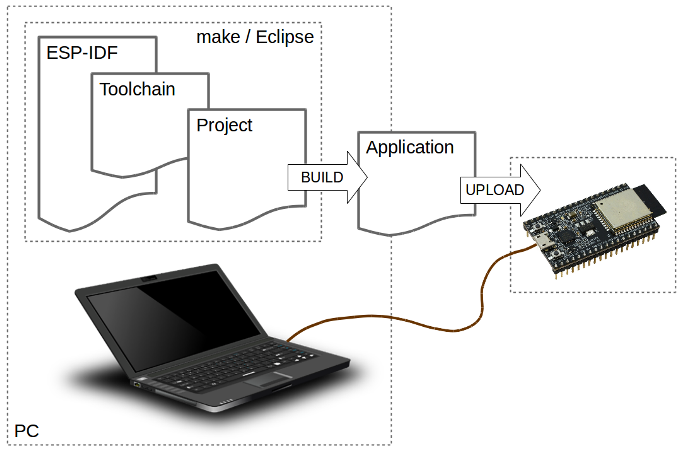
\includegraphics[scale=0.3]{Pictures/dev_setup.png}
    \caption{Typical Developer Setup}
    \label{fig:dev_setup}
\end{figure}

The PC, or the Development Host can be any of Linux, Windows or Mac. The ESP32 based development board is connected to the Development Host over a USB cable. The Development Host has the ESP-IDF (Espressif's SDK), the compiler toolchain and the code for your project. The development host builds this code and generates the executable firmware image. The tools on the Development Host then download the generated firmware image on to the development board. As the firmware executes on the development board, the logs from the firmware can be monitored from the Development Host.

\section{Getting ESP-Bootstrap}\index{Getting ESP-Bootstrap}

Let's get started by cloning the ESP-Bootstrap git repositories \url{https://github.com/mahavirj/esp-bootstrap}. This repository contains the sequence of applications that we will use for this exercise. This repository also contains a stable release version of IDF as a git submodule. This ensures that we are working off of a stable release of IDF.

\begin{verbatim}
$ git clone --recursive https://github.com/mahavirj/esp-bootstrap
\end{verbatim}

This repository already contains a copy of the IDF, Espressif's IoT Development Framework. Let's define the IDF\_PATH variable to point to the correction location of IDF. This can be done by executing the following command in your console:

\begin{verbatim}
$ export IDF_PATH=/path/to/esp-bootstrap/esp-idf
\end{verbatim}

Now let's make sure your development host (Windows, Linux or Mac) has the required packages to build and monitor ESP32 based projects. What you specifically need to do is:
\begin{itemize}
    \item Setting the toolchain \url{https://docs.espressif.com/projects/esp-idf/en/latest/get-started/#setup-toolchain}
    \item Establish serial connection with ESP32 \url{https://docs.espressif.com/projects/esp-idf/en/latest/get-started/establish-serial-connection.html}
\end{itemize}

\section{ESP-IDF}\index{ESP-IDF}

ESP-IDF is Espressif's IoT Development Framework. 
\begin{itemize}
    \item ESP-IDF is a collection of libraries and header files that provides the core software components that are required to build any software projects on ESP32. 
    \item ESP-IDF also provides tools and utilities that are required for typical developer and production usecases, like build, flash, debug and measure.
\end{itemize}

The IDF has a component-based design. 

\begin{figure}[h]
    \centering
    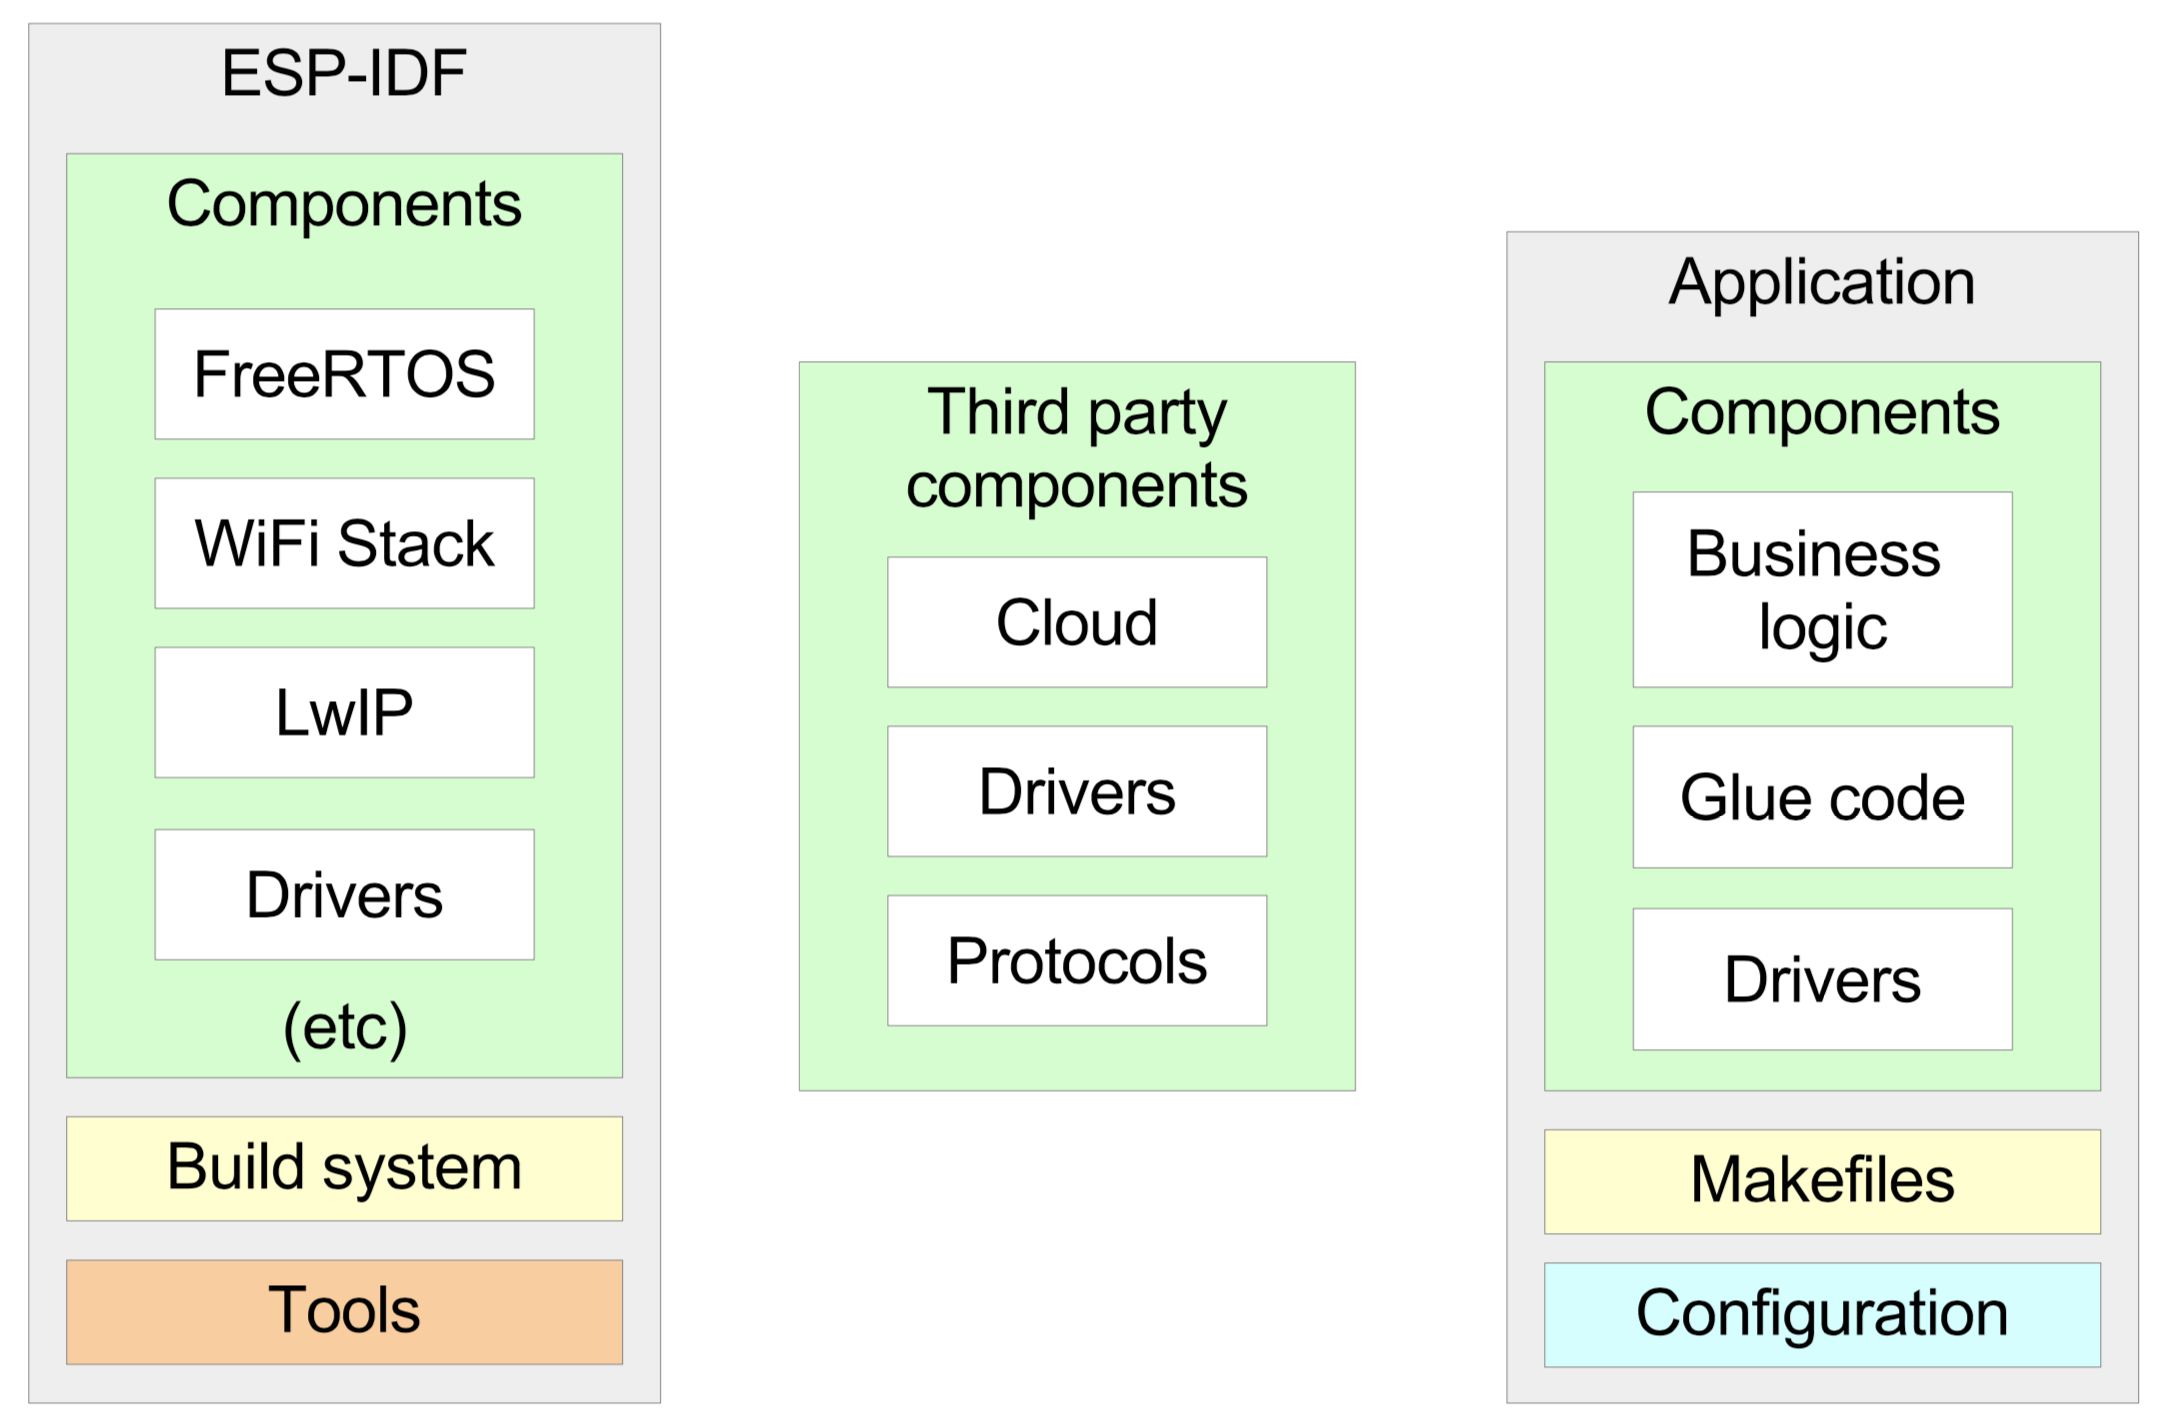
\includegraphics[width=\textwidth]{Pictures/idf_comp.png}
    \caption{Component Based Design}
    \label{fig:idf_comp_design}
\end{figure}

All the software in the IDF is available as components. The Operating System, the network stack, Wi-Fi drivers, middleware modules like the HTTP Server are all components within IDF. 

This design allows you to use your own or third-party components that are built for ESP-IDF.

A developer typically builds \textit{applications} against the IDF. The applications typically contains the business logic, any drivers for externally interfaced peripherals and the SDK configuration.

\begin{figure}[h]
    \centering
    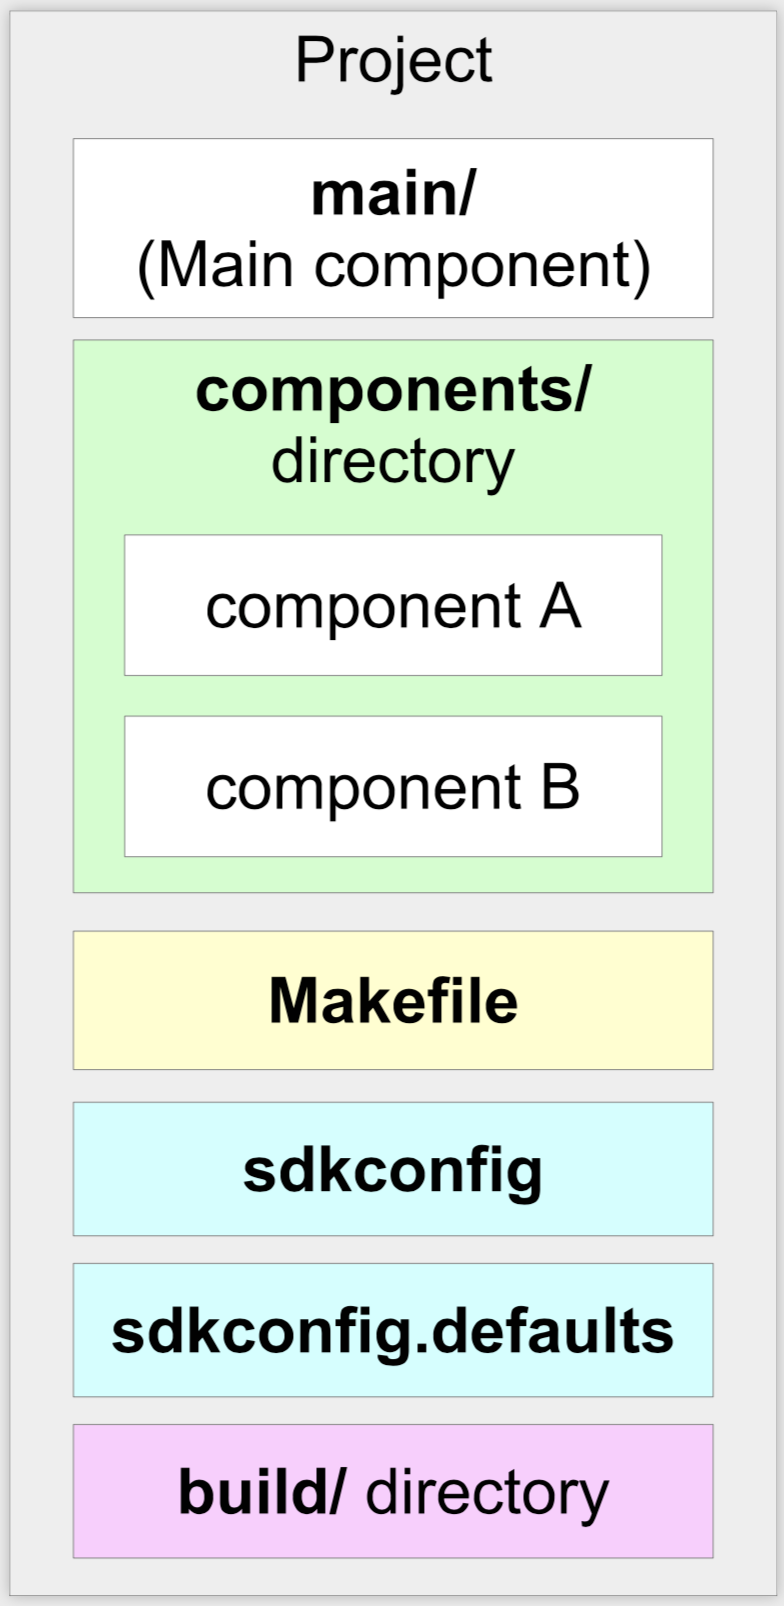
\includegraphics[scale=0.1]{Pictures/app_structure.png}
    \caption{Application's Structure}
    \label{fig:app_structure}
\end{figure}

An application must contain one \textit{main} component. This is the primary component that holds the application logic. The application may additionally include other components as may be desired.
The application's \textit{Makefile} defines the build instructions for the application. 
Additionally, an optional \textit{sdkconfig.defaults} may be placed that picks up the default SDK configuration that should be selected for this application. More details about the SDK configuration follow.

\subsection{SDK Configuration}\index{SDK Configuration}

Given that this is an embedded application with footprint constraints, the IDF allows every application to choose its own SDK configuration. The SDK configuration allows you to select specific configuration options of the SDK that suit your application.

Typically, there is a feature v/s footprint tradeoff, where pulling in a new feature will consume greater memory footprint.

Let us now first use the \textit{Hello World} application and launch the SDK configuration for this application.

\begin{verbatim}
$ cd esp-bootstrap/1hello_world
$ make -j8 menuconfig
\end{verbatim}

This will first open a pop-up screen for the SDK configuration.

For our current scenario, we will choose the default configuration. Later in this series, we will look at greater details into the SDK configuration options. For now, you can simply exit from this screen. On exiting, when asked for a prompt whether you want to save the SDK configuration, say "Yes".

\ksnotebox{If you are building the application for the first time, the SDK configuration screen will pop-up automatically even if you build for some other build target. For subsequent builds this SDK configuration screen wouldn't show up again unless you specify the \textit{menuconfig} target.}

\subsection{Build and Flash}\index{Build and Flash}
\begin{verbatim}
$ make -j8 flash monitor
\end{verbatim}

The SDK will then build the entire SDK and the application. Once the build is successful, it will write the generated firmware to the device.

At this point you should have connected the device to your development host. If you have installed the correct drivers, you should see a new device in your machine. For Windows, a new COM port would have been created. For Linux/OSX, a new file would appear in /dev/tty.*. The flashing utility should know which serial port is connected to your device. This can be configured by setting the 'ESPPORT' environment variable. The following command should help:
\begin{verbatim}
$ export ESPPORT=/dev/tty.SLAB_USBTOUART
\end{verbatim}

The rate at which the flashing utility writes firmware to the device can also be configured. This is called the baud rate. The typical rate is 115200. But this can be extended upto 921600. Let's configure the maximum baud rate for our flashing.
\begin{verbatim}
$ export ESPBAUD=921600
\end{verbatim}

\ksnotebox{On some development boards you may have to press a specific button configuration in order to put the development board into the 'flashing mode'. Please refer to your development board's documentation for these details. For ESP32-DevKit-C, no such button press is required, the board is automatically put into the flashing mode by the flasher utility.}

\section{The Code}\index{The Code}
Now let's look at the code of the Hello World Application. It is only a few lines of code as shown below:
\begin{minted}{c}
#include <stdio.h>
#include "freertos/FreeRTOS.h"
#include "freertos/task.h"


void app_main()
{
    int i = 0;
    while (1) {
        printf("[%d] Hello world!\n", i);
        i++;
        vTaskDelay(5000 / portTICK_PERIOD_MS);
    }
}
\end{minted}
The code is fairly simple. A few takeaways:
\begin{itemize}
\item The app\_main() function is the application entry point. All applications begin execution at this point. This function gets called after the FreeRTOS kernel is already executing on both the cores of the ESP32. Once FreeRTOS is initialis\
ed, it forks an application thread, called the main thread, on one of the cores. The app\_main() function is called in this thread's context. The stack of the application thread can be configured through the SDK configuration.
\item C library functions like printf(), strlen(), time() can be directly called. The IDF uses the newlib C library, which is a low-footprint implementation of the C library. Most of the category of functions of the C library like stdio, stdlib, string operations, math, time/timezones, file/directory operations are supported. Support for signals, locales, wchrs is not available. In our example above, we use the printf() function for printing to the console.
\item FreeRTOS is the operating system powering both the cores. FreeRTOS (https://www.freertos.org) is a tiny kernel that provides mechanisms for task creation, inter-task communication (sempahores, message queues, mutexes), interrupts and timers. In our example above, we use the vTaskDelay function for putting the thread to sleep for 5 seconds. Details of the FreeRTOS APIs are available at: https://www.freertos.org/a00106.html
\end{itemize}

\section{Progress so far}\index{Progress so far}
Now we have the basic development setup and process in place. We can build the code into executable firmware images. We can flash these images to a connected development board, and we can monitor the console to look at debug logs and messages generated by the firmware. 

Let's now build a simple power outlet with ESP32.

%----------------------------------------------------------------------------------------
%	CHAPTER 3
%----------------------------------------------------------------------------------------

\chapterimage{head2.png} % Chapter heading image

\chapter{The Outlet}

In this Chapter we will create a basic power outlet using the driver APIs of the ESP32. The power outlet will do the following:
\begin{itemize}
    \item Provide a button that the user can press
    \item Toggle an output GPIO on every button press
\end{itemize}
For the scope of this chapter, we won't worry about 'connectivity' of this power outlet. That will follow in subsequent chapters. Here we will only focus in implementing the outlet functionality. You may refer to the \textit{2outlet/} directory of esp-bootstrap for looking at this code. 

The code for the driver has been neatly isolated in the file \textit{app\_driver.c}. This way, later whenever you have to modify this application to adapt to your product, you could simply change the contents of this file to talk to your peripheral.

\section{The Push Button}\index{The Push Button}
Let's first create a push-button. The Devkit-C development board has a button called 'boot' which is connected to GPIO 0. We will configure this button to be used to toggle the outlet's state.

\ksnotebox{If you are developing with a different development board, please use the appropriate GPIO number for the button that this board may have.}

\subsection{The Code}\index{The Code}
The code for enabling this is shown as below:
\begin{minted}{c}
#include <iot_button.h>

button_handle_t btn_handle=iot_button_create(BUTTON_GPIO,
                                BUTTON_ACTIVE_LEVEL);
iot_button_set_evt_cb(btn_handle, BUTTON_CB_RELEASE,
                            push_btn_cb, "RELEASE");

\end{minted}

We use the \textit{iot\_button} module for implementing the button. 
First off we create the iot\_button object. We specify the GPIO number and the active level of the GPIO to detect the button press. In the case of DevKit-C the \textit{BUTTON\_GPIO} is set to GPIO 0. 

Then we register an event callback for the button, whenever the button is \textit{released} the \textit{\textbf{push\_btn\_cb}} function will be called. This function is called in the esp-timer thread's context. So do make sure that the default stack configured for the esp-timer thread is sufficient for your callback function.

The \textit{push\_btn\_cb} code then is simply as shown below:
\begin{minted}{c}
static void push_btn_cb(void* arg)
{
    static uint64_t previous;
    uint64_t current = xTaskGetTickCount();
    if ((current - previous) > DEBOUNCE_TIME) {
        previous = current;
        app_driver_toggle_state();
    }
}
\end{minted}

The \textit{xTaskGetTickCount()} is a FreeRTOS function that provides the current tick counts. In the callback function, we make sure that the button press doesn't accidentally generate multiple events in a short duration of time. This is generally not what the end-user wants. (In the current case, we absorb all events generated within a 300 millisecond span, and call it a single event.)
Finally, we call the function \textit{app\_driver\_toggle\_state()} which is responsible for toggling the output on or off.

\section{The Output}\index{The Output}
Now we will configure a GPIO to act as the output of the power outlet. We will assert this GPIO on or off which would ideally trigger a relay to switch the output on or off.

\subsection{The Code}\index{The Code}
First off we initialize the GPIO with the correct configuration as shown below:

\begin{minted}{c}
gpio_config_t io_conf;
io_conf.mode = GPIO_MODE_OUTPUT;
io_conf.pull_up_en = 1;
io_conf.pin_bit_mask = ((uint64_t)1 << OUTPUT_GPIO);

/* Configure the GPIO */
gpio_config(&io_conf);

\end{minted}

In this example, we have chosen GPIO 27 to act as the output. We initialize the \textit{gpio\_config\_t} structure with the settings to set this as a GPIO output with internal pull-up enabled.

\begin{minted}{c}
/* Assert GPIO */
gpio_set_level(OUTPUT_GPIO, target);

\end{minted}

Finally, the state of the GPIO is set using the \textit{gpio\_set\_level()} call.

\section{Progress so far}\index{Progress so far}
With this, now we have a power outlet functionality enabled. Once you build and flash this firmware, every time the user presses the push-button the output from the ESP32 toggles on and off. As of now, this is not a connected outlet though. 

As our next step, let's add Wi-Fi connectivity to this firmware.

%----------------------------------------------------------------------------------------
%	CHAPTER 4
%----------------------------------------------------------------------------------------

\chapterimage{band1.png} % Chapter heading image

\chapter{Connecting to Wi-Fi}
Let's now get this power outlet on a Wi-Fi network. In this Chapter we will connect to a hard-coded Wi-Fi network that is embedded within the device's firmware executable image. You may refer to the \textit{3wifi\_connection/} directory of esp-bootstrap for looking at this code.

Wi-Fi is a protocol that can generate asynchronous events like connectivity lost, connection established, DHCP Address received etc. For this, we register a handler with the Wi-Fi and network subsystem. This handler will get called whenever either of these asynchronous events occurs.

\section{The Code}\index{The Code}
\begin{minted}{c}
#include <esp_wifi.h>
#include <esp_event_loop.h>

tcpip_adapter_init();
esp_event_loop_init(event_handler, NULL);

wifi_init_config_t cfg = WIFI_INIT_CONFIG_DEFAULT();
esp_wifi_init(&cfg);
esp_wifi_set_mode(WIFI_MODE_STA);

wifi_config_t wifi_config = {
    .sta = {
        .ssid = EXAMPLE_ESP_WIFI_SSID,
        .password = EXAMPLE_ESP_WIFI_PASS,
    },
 };
esp_wifi_set_config(ESP_IF_WIFI_STA, &wifi_config);
esp_wifi_start();

\end{minted}

In the above code:
\begin{itemize}
    \item We initialize the TCP/IP stack with the \textit{tcpip\_adapter\_init()} call
    \item Similarly, the Wi-Fi subsystem and its station interface is initialized with the calls to \textit{esp\_wifi\_init()} and \textit{esp\_wifi\_set\_mode()}
    \item Finally, the hard-coded SSID and passphrase configuration of the target Wi-Fi network are configured and we start the station using a call to \textit{esp\_wifi\_start()}
\end{itemize}

The call to \textit{esp\_event\_loop\_init()} is important. The event loop collects events from the TCP/IP Stack and the Wi-Fi subsystem. It delivers these events to the callback that is registered through the first parameter.

\ksnotebox{The callback handler is executed from the event loop task. Care should be taken to ensure that this callback's execution doesn't overflow the event loop's stack. If you need a deeper stack in your callback, you can increase the event loop's stack size by changing the SDK configuration.}

The asynchronous event handler that is registered with the event loop can be implemented as:
\begin{minted}{c}
esp_err_t event_handler(void *ctx, system_event_t *event)
{
    switch(event->event_id) {
    case SYSTEM_EVENT_STA_START:
        esp_wifi_connect();
        break;
    case SYSTEM_EVENT_STA_GOT_IP:
        ESP_LOGI(TAG, "Connected with IP Address:%s",  
             ip4addr_ntoa(&event->event_info.got_ip.ip_info.ip));
        break;
    case SYSTEM_EVENT_STA_DISCONNECTED:
        esp_wifi_connect();
        break;
    return ESP_OK;
}
\end{minted}

The event handler current handles 3 events. When it receives an event \textit{SYSTEM\_EVENT\_STA\_START}, it asks the station interface to connect using the \textit{esp\_wifi\_connect()} call. The same action is taken even when we receive a Wi-Fi disconnect event.

The event \textit{SYSTEM\_EVENT\_STA\_GOT\_IP} is received when a DHCP IP address is obtained by ESP32. In this particular case, we  only print the IP address on the console.

\section{Progress so far}\index{Progress so far}
You can now modify the application to enter your Wi-Fi network's SSID and the passphrase. When you compile and flash this code on your development board, the ESP32 should connect to your Wi-Fi network and print the IP address on the console. The outlet's functionality of toggling the GPIO on pressing the push-button is, of course, also retained.

One problem with this approach is that the Wi-Fi settings are hard-coded into the firmware image. While this is ok for a hobby project, a product will require the end-user to dynamically configure this device with their settings. This is what we will look at in the next chapter.

%----------------------------------------------------------------------------------------
%	CHAPTER 5
%----------------------------------------------------------------------------------------

\chapterimage{head2.png} % Chapter heading image

\chapter{Network Configuration}

In this step we will build a firmware such that the end-user can configure her Wi-Fi network's credentials into the device at run-time. Since a user's network credentials will be stored persistently on the device, we will also provide a \textit{Reset to Factory} action where a user's configurations can be erased from the device.
You may refer to the \textit{4network\_config/} directory of esp-bootstrap for looking at this code.

In the previous example, we had hard-coded the Wi-Fi credentials into the firmware. This obviously doesn't work for a end-user product.

\section{Overview}\index{Overview}
As can be seen in this figure, in the network configuration stage, the end-user typically uses her smart-phone to \textit{securely} configure her Wi-Fi credentials into your device. Once the devices acquires these credentials, it can then connect to her home Wi-Fi network. 

\begin{figure}
    \centering
    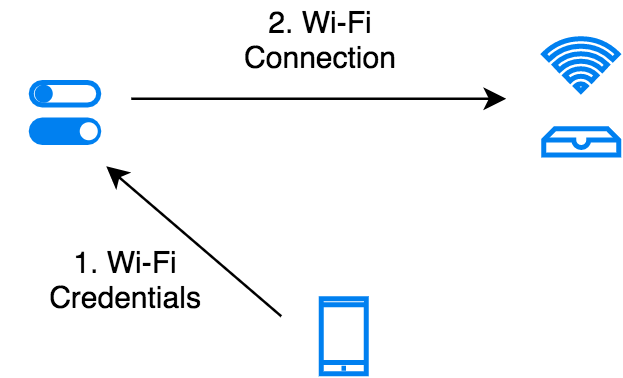
\includegraphics[scale=0.4]{Pictures/network_config.png}
    \caption{Network Configuration Process}
    \label{fig:network_config}
\end{figure}

There can be multiple channels through which your device can receive the Wi-Fi credentials. ESP32 supports the following mechanisms:

\begin{itemize}
    \item SoftAP 
    \item Bluetooth Low Energy (BLE)
    \item Smart-Config
\end{itemize}

Each of these have their own pros and cons. There is no single correct way of doing this, some developers may pick one way, and some the other, depending upon what you value more.

\subsection{SoftAP}\index{SoftAP}
In the SoftAP mechanism your outlet will launch its own temporary Wi-Fi Access Point. The user can then connect their smart-phones to this temporary Wi-Fi network. And then use this connection to transfer the Home Wi-Fi's credentials to the outlet. Many connected devices in the market today, like the Google Chromecast, Amazon's Echo use this kind of mechanism. In this network configuration workflow, the user has to 
\begin{itemize}
    \item switch their phone's Wi-Fi network to your outlet's temporary Wi-Fi network
    \item launch your phone application
    \item enter her home Wi-Fi credentials that will be then transferred to the outlet over the SoftAP connection
\end{itemize}
From a user experience perspective, the first step of this requires the user to change their phone's Wi-Fi network. This may be confusing to some users. Additionally, changing the Wi-Fi network programatically through the phone application may not always be possible (iOS and some variants of Android don't allow application to this). The advantage of this method though is that it is very reliable (SoftAP being just Wi-Fi is an established mechanism), and doesn't require a lot of additional code (since it's all over Wi-Fi).

\subsubsection{Apple's WAC}\index{Apple's WAC}
Apple's Wireless Accessory Configuration (WAC) protocol also uses the SoftAP mechanism for transferring credentials. But in this case, iOS itself manages the switching of Wi-Fi networks between the device's network and the user's home network. Since this support is embedded within iOS itself, this offers a much smoother user experience.
One point to note though is that Apple's WAC configuration mechanism mandates that your device, the outlet, should have Apple's security co-processor (a chip) embedded on your board. So the simplified user experience comes at the cost of having another chipset embedded within your board design.

\subsection{BLE}\index{BLE}

In the Bluetooth Low Energy (BLE) method, your outlet will be doing a BLE advertisement. Phones in the vicinity can see this advertisement, and ask the user to do a BLE connection with your device. Then this network is used to transfer the credentials to the outlet.
In this network configuration workflow, the user doesn't have to do the hard task of switching between Wi-Fi networks. Additionally, both iOS and Android allow phone application to scan for BLE devices in the vicinity and also connect to them through the app. This means a much smoother end-user experience.

One side-effect, though, of using the BLE based network configuration is that it also pulls in the code for Bluetooth. This means your flash requirement may be affected since your firmware size will increase. During the network configuration mode, BLE will also consume memory until the network configuration is complete.

\subsection{Smart-Config}\index{Smart-Config}
XXX

\section{Network Configuration with ESP}\index{Network Configuration with ESP}

Espressif provides a \textbf{Unified Provisioning} module for assisting you with your network configuration. The following components are offered:
\begin{itemize}
    \item \textbf{Unified Provisioning Specification:} A specification to \textit{securely} transfer Wi-Fi credentials to the device, independent of the transport (SoftAP, BLE)
    \item \textbf{IDF Components:} Software modules that implement this specification in the device firmware, available through ESP-IDF
    \item \textbf{Phone Libraries:} Reference implementations on iOS and Android are available that can be directly incorporated into your existing phone applications
    \item \textbf{Reference Phone Applications:} Fully functional Phone applications on Android and iOS are available for testing during your development, or for skinning with your brand's elements.
\end{itemize}
%----------------------------------------------------------------------------------------
%	CHAPTER 6
%----------------------------------------------------------------------------------------

\chapterimage{band1.png} % Chapter heading image

\chapter{Remote Control (Cloud)}

%----------------------------------------------------------------------------------------
%	CHAPTER 7
%----------------------------------------------------------------------------------------

\chapterimage{head2.png} % Chapter heading image

\chapter{Firmware Upgrades}

%----------------------------------------------------------------------------------------
%	CHAPTER 8
%----------------------------------------------------------------------------------------

\chapterimage{band1.png} % Chapter heading image

\chapter{Manufacturing}

\clearpage
\vspace*{\fill} 
\centering \Huge {\textit{Happy Productising!}}
\vspace*{\fill} 

\end{document}